% Figure 1 -- the learned emulator, one simulated year. Compile: pdflatex fig01_overview.tex
\documentclass[tikz,border=3pt]{standalone}
\usepackage[scaled=0.92]{helvet}
\renewcommand{\familydefault}{\sfdefault}
\usepackage{amsmath}
\usetikzlibrary{positioning,arrows.meta,fit,backgrounds,calc,shapes.geometric}
\definecolor{emu}{HTML}{2A78D6}
\definecolor{emul}{HTML}{CDE2FB}
\definecolor{emuxl}{HTML}{EEF5FD}
\definecolor{orig}{HTML}{222220}
\definecolor{ink2}{HTML}{52514E}
\definecolor{aqua}{HTML}{1BAF7A}
\definecolor{aqual}{HTML}{D6F2E8}
\definecolor{orng}{HTML}{EB6834}
\definecolor{orngl}{HTML}{FCE3D8}
\definecolor{viol}{HTML}{6250D6}
\definecolor{violl}{HTML}{E4E0F8}
\definecolor{grey}{HTML}{F0EFEC}
\definecolor{greyd}{HTML}{8A8984}
\tikzset{
  box/.style={draw=#1, fill=#1!12, rounded corners=2pt, line width=0.6pt, align=center, inner sep=3pt,
              font=\scriptsize\linespread{0.95}\selectfont, text=orig},
  hdr/.style={font=\footnotesize\bfseries, text=orig},
  note/.style={font=\tiny, text=ink2, align=left},
  arr/.style={-{Stealth[length=4pt]}, line width=0.7pt, draw=ink2},
  fb/.style={-{Stealth[length=4pt]}, line width=0.9pt, draw=orng, dashed},
}
\begin{document}
\hyphenpenalty=10000\exhyphenpenalty=10000
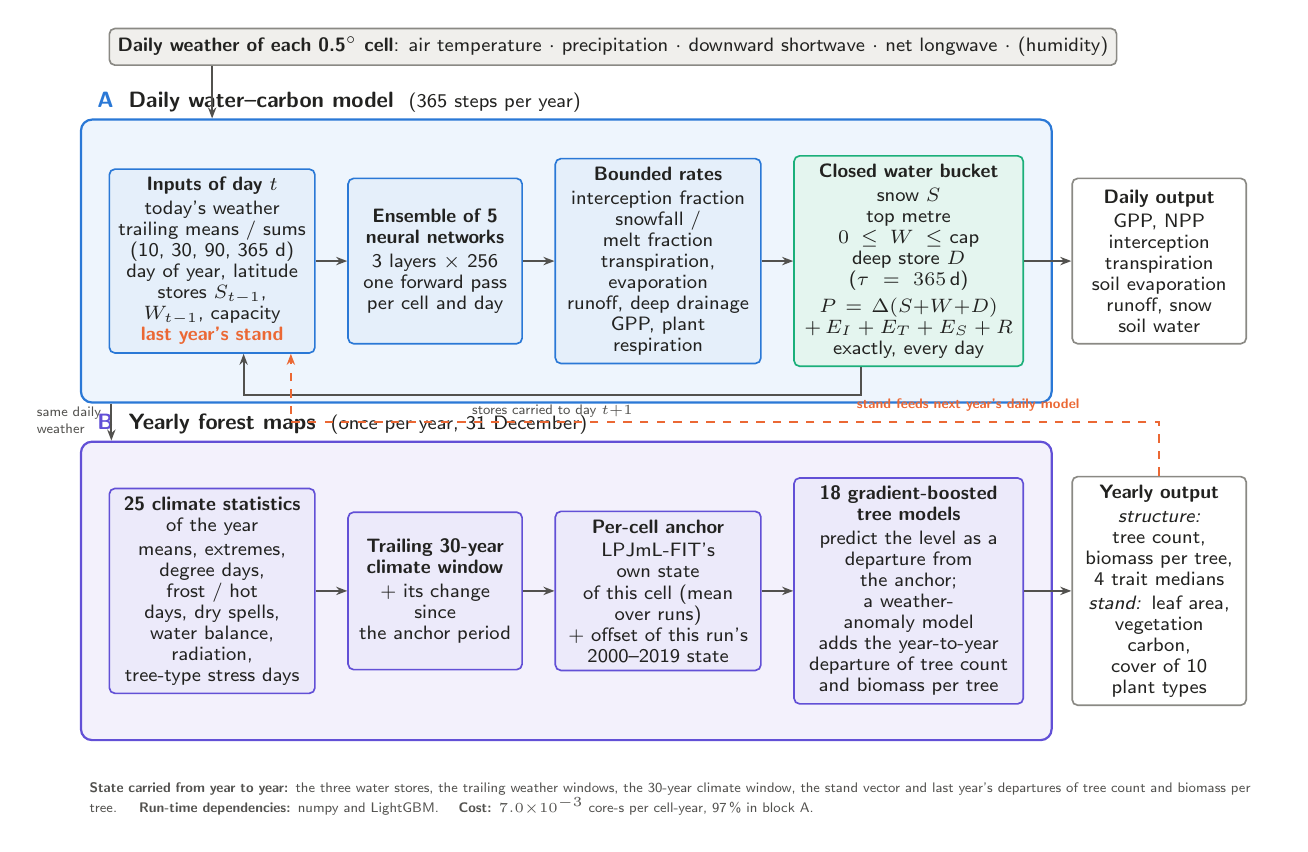
\begin{tikzpicture}[node distance=4mm and 4mm]
% ---------------- input
\node[box=greyd, minimum width=120mm, fill=grey] (wx) {\textbf{Daily weather of each 0.5$^\circ$ cell}: air temperature $\cdot$ precipitation $\cdot$ downward shortwave $\cdot$ net longwave $\cdot$ (humidity)};

% ---------------- daily block
\node[box=emu, below=13mm of wx.south west, anchor=north west, minimum width=25mm, minimum height=21mm,
      text width=24mm] (feat) {\textbf{Inputs of day $t$}\\[1pt]
  today's weather\\ trailing means / sums\\ (10, 30, 90, 365 d)\\ day of year, latitude\\
  stores $S_{t-1}$, $W_{t-1}$, capacity\\ \textcolor{orng}{\textbf{last year's stand}}};
\node[box=emu, right=4mm of feat, minimum width=21mm, minimum height=21mm, text width=20mm] (net)
  {\textbf{Ensemble of 5\\ neural networks}\\[1pt] 3 layers $\times$ 256\\ one forward pass\\ per cell and day};
\node[box=emu, right=4mm of net, minimum width=25mm, minimum height=21mm, text width=24mm] (heads)
  {\textbf{Bounded rates}\\[1pt] interception fraction\\ snowfall / melt fraction\\ transpiration, evaporation\\
  runoff, deep drainage\\ GPP, plant respiration};
\node[box=aqua, right=4mm of heads, minimum width=28mm, minimum height=21mm, text width=27mm] (bucket)
  {\textbf{Closed water bucket}\\[1pt] snow $S$\\ top metre $0\le W\le$ cap\\ deep store $D$ ($\tau = 365$\,d)\\[2pt]
  $P = \Delta(S{+}W{+}D)$\\ $+\,E_I + E_T + E_S + R$\\ exactly, every day};
\draw[arr] (feat) -- (net);
\draw[arr] (net) -- (heads);
\draw[arr] (heads) -- (bucket);
\draw[arr] ($(bucket.south)+(-6mm,0)$) -- ++(0,-3.5mm) -| node[pos=0.25, below, note]{stores carried to day $t{+}1$} ($(feat.south)+(4mm,0)$);
\begin{scope}[on background layer]
  \node[draw=emu, fill=emuxl, rounded corners=4pt, line width=0.8pt, inner sep=3.5mm, inner ysep=4.5mm,
        fit=(feat)(net)(heads)(bucket)] (dailyblk) {};
\end{scope}
\node[hdr, anchor=south west] at ($(dailyblk.north west)+(1mm,-0.5mm)$) {\textcolor{emu}{A}\; Daily water--carbon model \;\textmd{\scriptsize(365 steps per year)}};
\draw[arr] (wx.south -| feat.north) -- ++(0,0) -- (feat.north |- dailyblk.north);

% daily outputs
\node[box=greyd, fill=white, right=6mm of bucket, minimum width=21mm, text width=20mm, minimum height=21mm] (dout)
  {\textbf{Daily output}\\[1pt] GPP, NPP\\ interception\\ transpiration\\ soil evaporation\\ runoff, snow\\ soil water};
\draw[arr] (bucket) -- (dout);

% ---------------- yearly block
\node[box=viol, below=17mm of feat.south west, anchor=north west, minimum width=25mm, minimum height=20mm,
      text width=24mm] (stats) {\textbf{25 climate statistics}\\ of the year\\[1pt] means, extremes, degree days,\\
  frost / hot days, dry spells,\\ water balance, radiation,\\ tree-type stress days};
\node[box=viol, right=4mm of stats, minimum width=21mm, minimum height=20mm, text width=20mm] (win)
  {\textbf{Trailing 30-year\\ climate window}\\[1pt] + its change since\\ the anchor period};
\node[box=viol, right=4mm of win, minimum width=25mm, minimum height=20mm, text width=24mm] (anc)
  {\textbf{Per-cell anchor}\\[1pt] LPJmL-FIT's own state\\ of this cell (mean over runs)\\ + offset of this run's\\ 2000--2019 state};
\node[box=viol, right=4mm of anc, minimum width=28mm, minimum height=20mm, text width=27mm] (gbm)
  {\textbf{18 gradient-boosted\\ tree models}\\[1pt] predict the level as a\\ departure from the anchor;\\ a weather-anomaly model\\ adds the year-to-year\\ departure of tree count\\ and biomass per tree};
\draw[arr] (stats) -- (win);
\draw[arr] (win) -- (anc);
\draw[arr] (anc) -- (gbm);
\begin{scope}[on background layer]
  \node[draw=viol, fill=violl!45, rounded corners=4pt, line width=0.8pt, inner sep=3.5mm, inner ysep=4.5mm,
        fit=(stats)(win)(anc)(gbm)] (yearblk) {};
\end{scope}
\node[hdr, anchor=south west] at ($(yearblk.north west)+(1mm,-0.5mm)$) {\textcolor{viol}{B}\; Yearly forest maps \;\textmd{\scriptsize(once per year, 31 December)}};
\node[box=greyd, fill=white, right=6mm of gbm, minimum width=21mm, text width=20mm, minimum height=20mm] (yout)
  {\textbf{Yearly output}\\[1pt] \emph{structure:} tree count,\\ biomass per tree,\\ 4 trait medians\\[1pt]
  \emph{stand:} leaf area,\\ vegetation carbon,\\ cover of 10 plant types};
\draw[arr] (gbm) -- (yout);
% weather to stats
\draw[arr] ($(dailyblk.south west)+(4mm,0)$) -- node[left, note, pos=0.45]{same daily\\ weather} ($(yearblk.north west)+(4mm,0)$);

% feedback: stand -> next year's daily model, routed through the gap between the two blocks
\coordinate (gapy) at ($(dailyblk.south)!0.5!(yearblk.north)$);
\draw[fb] (yout.north) -- (yout.north |- gapy) -- node[pos=0.22, above, font=\tiny\bfseries, text=orng]{stand feeds next year's daily model} ($(feat.south |- gapy)+(10mm,0)$) -- ($(feat.south)+(10mm,0)$);

% legend / state carried
\node[note, below=4mm of yearblk.south west, anchor=north west, text width=150mm] (st)
  {\textbf{State carried from year to year:} the three water stores, the trailing weather windows, the 30-year climate window,
  the stand vector and last year's departures of tree count and biomass per tree. \quad \textbf{Run-time dependencies:} numpy and LightGBM. \quad
  \textbf{Cost:} $7.0{\times}10^{-3}$ core-s per cell-year, 97\,\% in block A.};
\end{tikzpicture}
\end{document}
